%!TEX root = p.tex
\section{Data Pipeline}
In order to provide rich plots of the importance of topics over time, it is necessary to parse the full text of the documents.  The two most important features to extract are word stem occurrences and named entity instances.  The ability to determine the set of relevant documents that contain specific entities or terms is the fundamental building block of our topic visualization.  Rather than try to extract topics using machine learning algorithms, our approach is to provide interactive visual query building elements which enable the user to quickly construct an expression which will allow for targeted exploration of the content of a full text corpus.

Interactive query building implies a system which is capable providing feedback to the user about what query terms might be interesting to add to an expression.  The terms of interest for the purposes of news exploration will commonly be named entities.  For example, one might wish filter the documents down to a set that contain the word �election�, inspect the list of people who appear in those documents, and plot the frequency of mentions for specific presidential candidates in order to assess the interplay of reporting and the election process.   Exploring the mechanics of this query building work flow leads to a few specific queries that must be supported.
- What are all the documents that contain a word derived from stem �xyz�?
- What are all the documents that contain a specific named entity?
- What are the most important entities mentioned over a specific set of documents?
- What are all the documents that contain a combination of terms, possibly filtered by other features, such as date, page, or publication?
- Given that the user has typed �abc�, what other terms might they want to include?

\begin{figure}[htb]
  \centerline{
    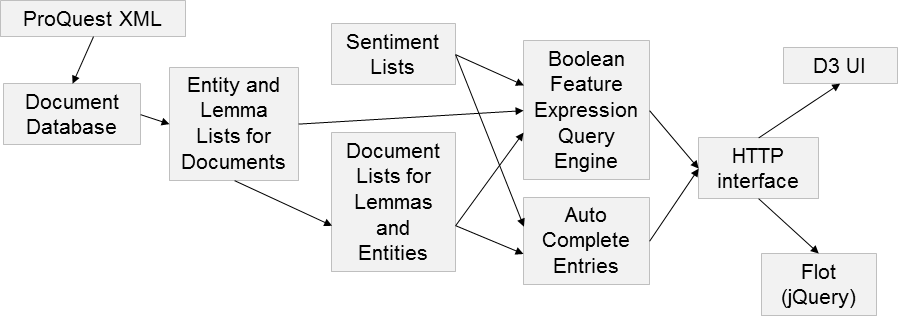
\includegraphics[scale=0.28]{figures/pipeline.png}
  }
  \caption{The overall data processing pipeline. The document, entity, and lemma lists are all computed off-line.}
  \label{fig:pipeline}
\end{figure}

Servicing these queries in real-time requires pre-computation of several indexes to provide a responsive user experience.  The process of extracting entities and lemmas from the full-text documents alone requires 18 hours of processing time when performed on a Core i7 i920 processor (2.9GHz. 4-core, 8 threads).  Unfortunately handling of advanced queries against the data restricts the type of offline processing that can be used.  A user might create a query which selects an arbitrary set of documents and request the most important named entities contained within those documents.  Thus, the data need to be stored in a format that supports efficient aggregation.   

Our processing pipeline consists of several phases.  First, the metadata and full-text fields are extracted from the original ProQuest XML dump using XPath expression.  These fields are stored in a SQL database.  Next, the Stanford CoreNLP tools are run over the corpus to extract word stems, parts of speech, named entity terms, and named entity classes.  A unique id is allocated for word form and entity and the full this mapping is recorded in another pair of SQL tables.  Simultaneously, packed and sorted lists of hit counts are produced for the input documents, e.g. word\#1 - 10 hits - word \#5 - 20 hits - word\#1000 - 1 hit.   One row per document containing the list is stored in the SQL database.  Later, these lists will be rapidly aggregated by the query engine to compute the most important terms over a document collection.

After the full-text has been converted into term hit lists, the lists are transformed so that they can be queried in the other direction.  For each entity or word stem, one row is inserted into the database that has a packed list of documents and the frequency of the term within those documents.  These are packed and sorted just like the previous hit lists, e.g. document\#20 - 5 hits, document \#100 - 1 hit, document \#253 - 3 hits.   The query engine aggregates these lists to determine the set of documents which match a query provided by the user.  

Sentiment lists extracted from the General Inquirer database are also imported to allow for online sentiment analysis from the visualization.  The sentiments are lists of word stems, so the same code that processes normal user queries can expand the sentiments terms into set of word terms.

Once the core inputs to the query engine have been generated, potential auto-complete candidates are computed.  Auto-complete is handled by doing a simple prefix query on an SQL table that contains mappings between input words and potential completion word stems, entities, or sentiment names.  Each candidate completion is assigned a score based on its global frequency in the data set; the SQL database sorts the candidates by this score so that the most likely or interesting completions are presented to the user.  Since named entities may contain several words including unimportant honorifics, each individual word in an entity is used as an auto-complete key.  